\section{Architecture}
Before implementing the software system, it is a good idea to have a general overview of how the various parts of the system are connected.
In order to gain this overview, an overall architecture diagram was drawn.
\begin{figure}[h]
	\centering
	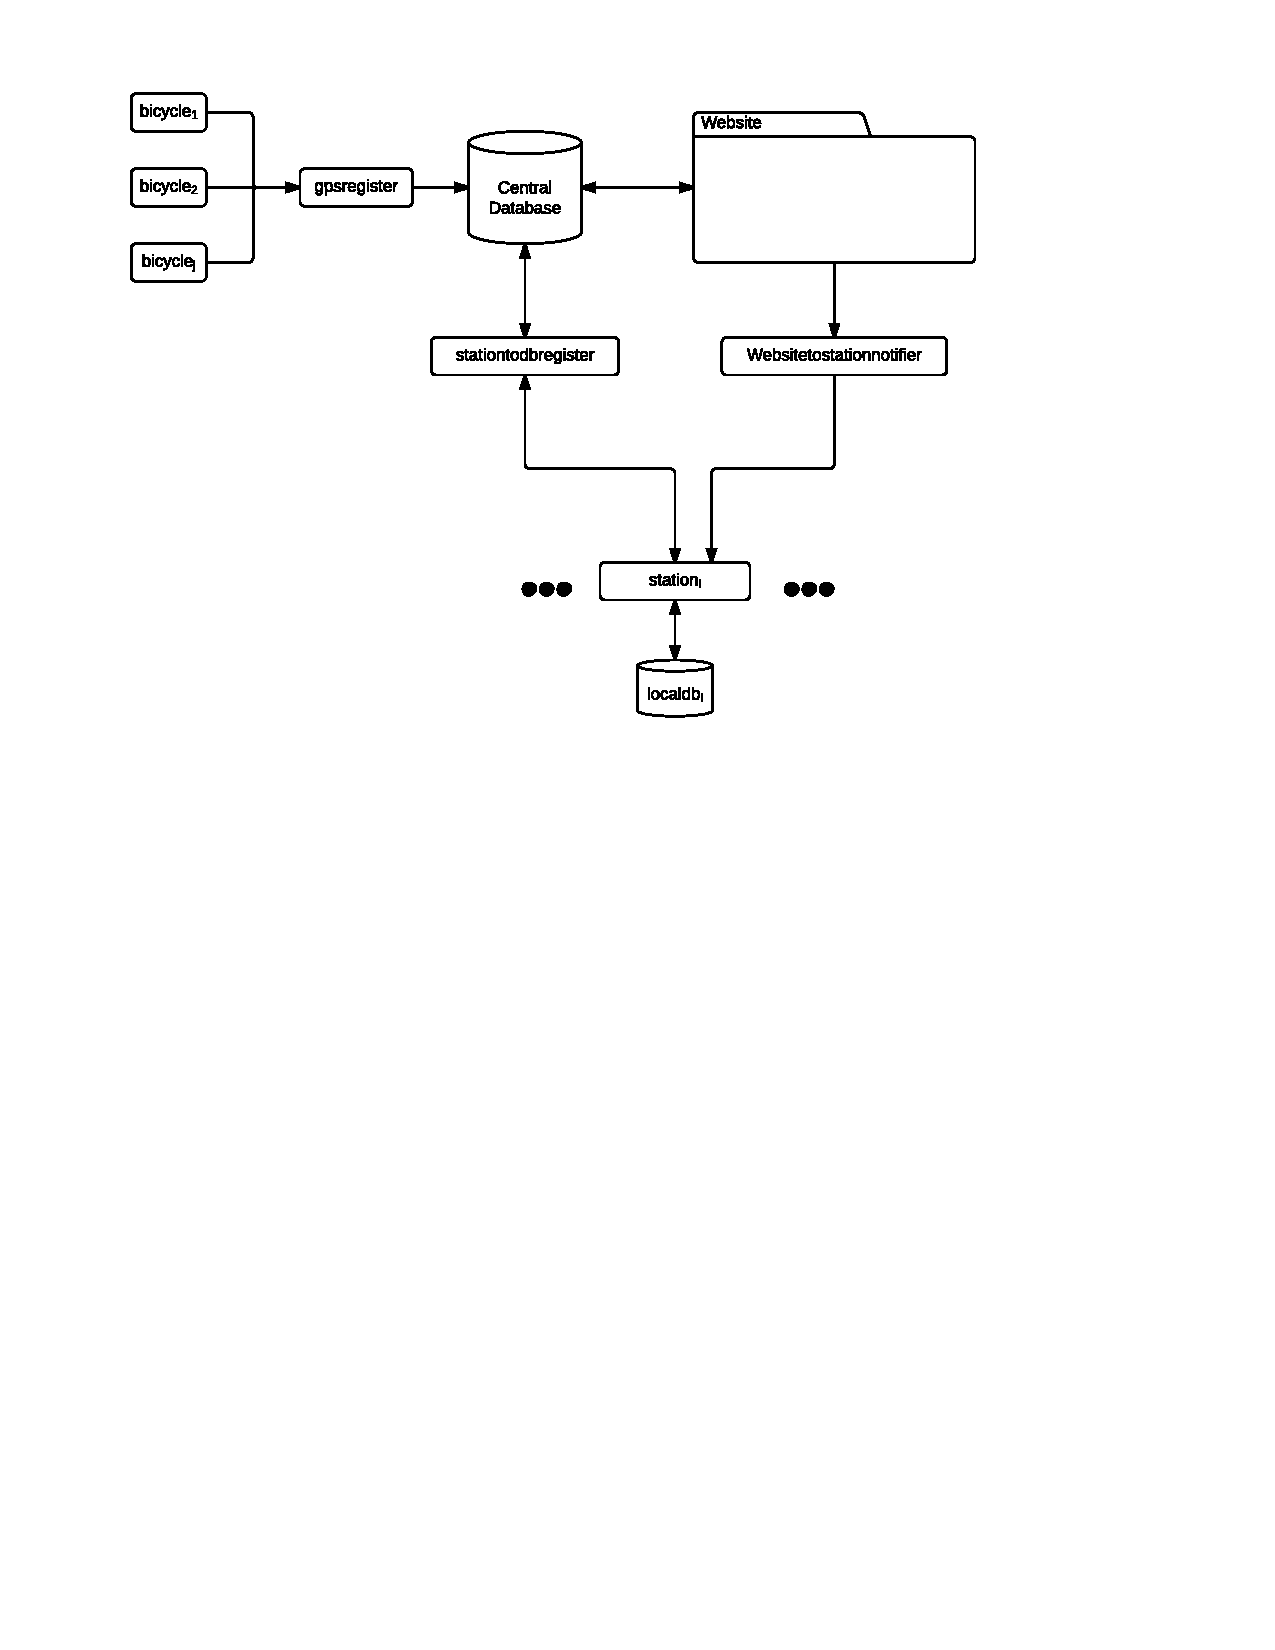
\includegraphics[trim=2cm 15.5cm 5cm 0cm, clip, scale=0.9]{design/architecture}
	\caption{Overall architecture}\label{fig:overallarch}
\end{figure}

It was found that the overall architecture should be as seen in \figref{fig:overallarch}.
In the illustration a single arrow is a one way communication, whereas two arrows are two way communication.
The architecture is very similar to a client-server pattern, where the central database is the server, and the stations and bicycles are the clients.
As we have a central booking system, and multiple simultaneous access points, the client-server pattern is found favourable.

As can be seen from the figure, the architecture consists of a central database as well as a website and three interfaces, where two of them contacts the central database.
Additionally, multiple stations and their associated local database exists.
The reason each station needs to have its own local database, and not merely use the central one is to minimize the necessary network communication, as well as allowing the stations to remain operational in case of network failure.
As of such, the local databases contains a subset of the central database, corresponding to the data involving the given station.

Additionally, the three interfaces each serves a function, as described here.
The gpsregister interface, is provided for the bicycles to register their current position in the central database, as well as logging its path in another table.
This data provided can be used for route mapping and positioning of bicycles.

The stationtodbregister interface serves the purpose of orienting the central database of changes performed at the local stations. Furthermore, it enables the local stations to read their subset of the central database, which is used for booting of stations from scratch, when their local database is empty.

The websitetostationnotifier is a little different, in that it is an interface provided to the website, such that when the website changes data, e.g. create a booking, the involved station is notified by the interface.

For the website part of the architecture, it is structured according to the MVC pattern, see \secref{sec:mvc}.
A detailed overview of the architecture of the controller and model part of the website are provided in \appref{app-arch:controller} and \appref{app-arch:model}

%stationer skal have egen database
%forklaring af figur
%husk teori og fancy ord, SOAP webservice er et eksempel

%uddybbelse af de enkelte komponenter.